% Chapter X

\chapter{Existing Heat Flux Partitioning Models} % Chapter title

\label{ch:name} % For referencing the chapter elsewhere, use \autoref{ch:name} 

%----------------------------------------------------------------------------------------

\section{Kurul \& Podowski (1990)}


In their original work published in 1990, Kurul \& Podowski \cite{kurul_1990} proposed a complete closure for the wall heat flux partitioning. They considered the applied heat flux to be divided between three mechanisms:

\begin{itemize}
\item A liquid single-phase heat flux $\phi_{c,L}$ ;
\item A boiling heat flux $\phi_{e}$ ;
\item A quenching heat flux $\phi_{q}$ induced by bubbles leaving the surface.
\end{itemize}

The total wall heat flux being :

\begin{align}
\phi_{w}=\phi_{c,L}+\phi_{e}+\phi_{q}
\end{align}

The convective heat flux is expressed as :
\begin{align}
\phi_{c,l}=A_{c,L} \rho_{L} c_{p,L}U_{L,\delta} \St_{L,\delta}\parth{T_{w}-T_{L,\delta}}
\label{eq:HFP_KP_phiCL}
\end{align}
with $\delta$ a location in the buffer layer.

Assuming bubbles are spherical and leave the surface at diameter $D_{lo}$, they write:
\begin{align}
\phi_{e}=\frac{1}{6}\pi {D_{lo}}^{3}\rho_{V}h_{LV}fN_{sit}\\
\label{eq:HFP_KP_phiE}
\end{align}

The quenching heat flux occurring over the wait time $t_{w}$ between two nucleated bubbles is computed as:  
\begin{align}
\phi_{q}=t_{w}fA_{q}\frac{2\lambda_{L}\parth{T_{w}-T_{L,\delta}}}{\sqrt{\pi \eta_{L} t_{w}}}
\label{eq:HFP_KP_phiQ}
\end{align}

This expression corresponds to the average heat flux for semi-infinite conduction over a time $t_{w}$, as expressed by Del Valle and Kenning \cite{DelValle}.

They also estimate the portion of the surface affected by the bubbles as:

\begin{align}
A_{q}=\mathrm{min}\parth{1\ ;\ F_{A}\pi R_{lo}^{2} N_{sit}}=1-A_{c,L}
\label{eq:HFP_KP_AQ}
\end{align}
where $F_{A}=4$ accounts for the bubble influence area when leaving the surface.

\npar

\textbf{\underline{Needed closure relationships : }} $N_{sit}$, $f$, $t_{w}$, $D_{lo}$ 

%------------------------------------------------

\section{Basu (2000)}

In 2005, Basu \etal \cite{Basu2005, Basu2005a} proposed a new HFP model together with a series of experiments to further study the different needed closure relationships. This model was meant to account for finer descriptions of the multiple phenomena at stake in subcooled flow boiling. In particular, they account for bubble sliding and merging and thus distinguish bubble departure diameter $D_{d}$ (leaving the nucleation site) and lift-off diameter $D_{lo}$ (leaving the wall).

Their approach consist of separating the boiling flow in three regions (Figure \ref{fig:Basu_zones}):

\begin{itemize}
\item Pre-ONB zone, where only liquid forced convection occurs, yielding:

\begin{equation}
\phi_{w}=h_{c,L} \parth{T_{w}-T_{L}}
\label{eq:HFP_B_preONB}
\end{equation}

\item Zone between the ONB and the OSV, prior to observing a net amount of vapor with bubble lifting off the surface. The heat flux is then still totally transferred to the liquid, but the equivalent convective heat transfer coefficient is enhanced due to the presence of bubbles on the wall:

\begin{equation}
\phi_{w}=\overline{h_{c,L}} \parth{T_{w}-T_{L}}
\label{eq:HFP_B_postONB}
\end{equation}

\item Post-OSV zone, where bubbles now leave the surface towards the bulk flow. This is where the other parts of the HFP appear \ie the boiling and quenching fluxes.
\end{itemize}


\begin{figure}[h]
\centering
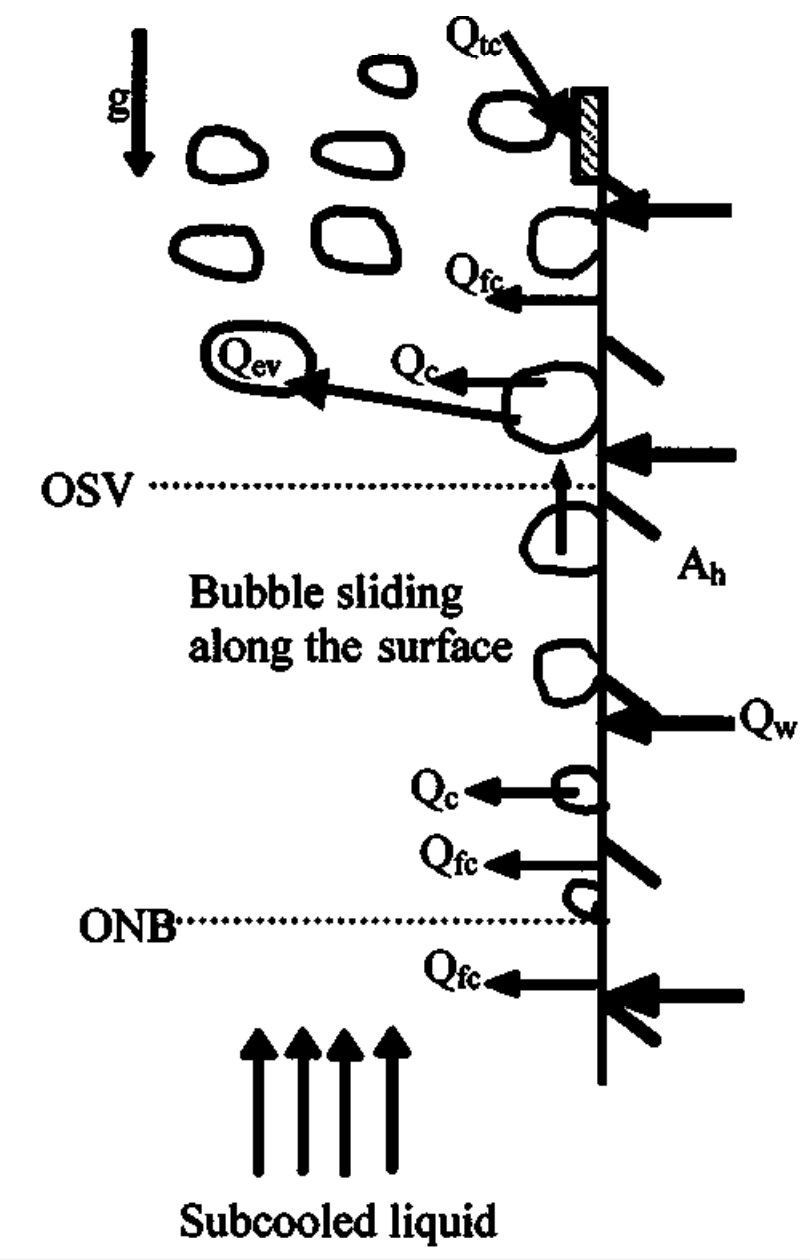
\includegraphics[width=0.5\linewidth]{img/HFP/Basu/zones.PNG}
\caption{Sketch of the heat transfers zones considered by Basu \etal. (Adapted from \cite{Basu2005})}
\label{fig:Basu_zones}
\end{figure}
	

The hypothesis of Basu \etal is that the heat flux is first transferred to the superheated liquid close to the wall (by convection and transient quenching), part of which contributing to the evaporation through the liquid-vapor interface. The remaining heat is transferred to the bulk liquid ($\phi_{L}$) either from the superheated liquid layer or bubble condensation. The whole heat transfer mechanism can thus be written as:

\begin{equation}
\phi_{w} = \phi_{c,L}+\phi_{q} = \phi_{e} + \phi_{L}
\label{eq:HFP_B_tot}
\end{equation}

In order to estimate the quenching heat flux associated to bubble sliding and lift-off, Basu \etal consider two cases: 

\begin{itemize}
\item[1] Bubble sliding from departure ($D=D_{d}$) to lift-off ($D=D_{lo}$) ;
\item[2] Bubble coalescence with neighboring sites before departure.
\end{itemize} 

Those two cases are distinguished using the average distance between nucleation sites $s$, which they suppose equal to $1/\sqrt{N_{sit}}$.

\subsection{Case 1 : Bubble sliding, $D_{d}<s$}

In this situation, the bubble will grow up to its departure diameter $D_{d}$ and slide over a length $l_{sl,0}$ before lifting-off. If $l_{sl,0}<s$, the bubble will slide up to its lift-off diameter $D_{l}$ and leave the wall withouth colliding with other bubbles. On the contrary, if $l_{sl,0}>=s$ the sliding bubble will merge with bubbles growing on their nucleation site, inducing a sudden growth of the bubble diameter that can exceed $D_{lo}$ and thus lift-off after sliding over a reduced length $l_{sl}<l_{sl,0}$. Those assumptions are summarized on Figure \ref{fig:Basu_sliding}.

\begin{figure}[h]
\centering
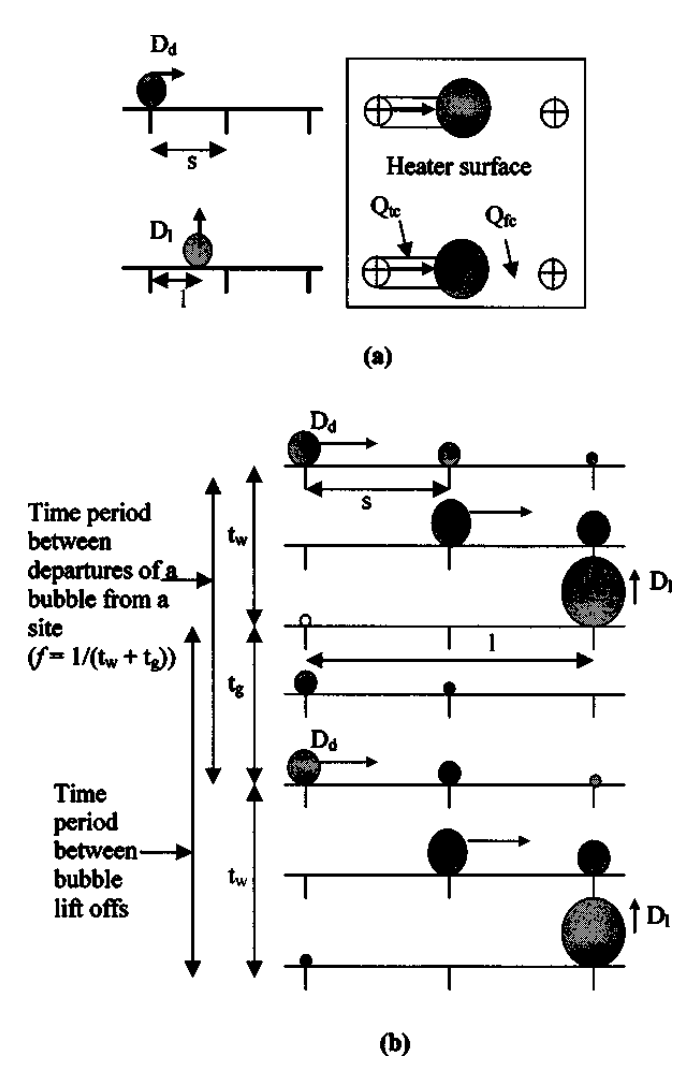
\includegraphics[width=0.5\linewidth]{img/HFP/Basu/slide.PNG}
\caption{Sliding bubble behavior considered by Basu \etal. (Adapted from \cite{Basu2005})}
\label{fig:Basu_sliding}
\end{figure}
	

If bubble coalescence occurs, the number of bubbles lifting-off the surface is lower than the actual number of nucleating sites. Basu \etal thus define a reduction factor:

\begin{align}
R_{f}&=
\begin{cases}
\dfrac{s}{l_{sl}} = \dfrac{1}{l\sqrt{N_{sit}}} & \text{if } l_{sl,0} \geq s \\
1 & \text{if } l_{sl,0}<s
\end{cases}
\end{align}  


Regarding bubble sizes, they suppose that bubbles coalesced by a sliding bubble while growing have a diameter $D_{d}$ \ie they were close to departure (in reality, the coalesced bubble would have a diameter $D<D_{d}$). This results in a bubble of diameter $D=\parth{D_{sl}^{3} + D_{d}^{3}}^{1/3}$ which will lift-off id $D>D_{lo}$. Consequently, a sliding bubble can merge with numerous bubbles before lifting off. Noting $N_{merg}$ the number of coalesced bubble and $D_{N}$ the resulting bubble diameter, the sliding distance is:

\begin{equation}
l_{sl}=N_{merg}s + l_{D_{N}\rightarrow D_{lo}}
\end{equation}
where $l_{D_{N}\rightarrow D_{lo}}$ is the remaining distance to slide if $D_{N}<D_{lo}$, being $0$ if $D_{N}>D_{lo}$.

The surface swiped by the sliding bubble is then expressed as $A_{sl} = C\overline{D}l_{sl}$ with $\overline{D}$ the average bubble diameter during sliding and $C$ the ration between the bubble diameter and its foot. After observing in their experiments that $D_{d}\approx 0.5D_{lo}$, Basu \etal choose:

\begin{equation}
\overline{D}=\frac{D_{lo}+D_{d}}{2}\approx 0.75D_{lo}
\end{equation}

Noting $t^{*}=\parth{\dfrac{\lambda_{L}}{h_{c,L}}}^{2} \dfrac{1}{\pi \eta_{L}}$ the time at which transient conduction heat transfer becomes equal to forced liquid convection, the quenching heat flux is expressed as:

\begin{equation}
\phi_{q} = \frac{1}{t_{w}+t_{g}} \int_{0}^{T}\frac{\lambda_{L}}{\sqrt{\pi \eta_{L}t}}\parth{T_{w}-T_{L}}A_{sl}R_{f}N_{sit}dt
\end{equation}
where $T=t^{*}$ if $t^{*}<t_{w}+t_{g}$ (forced convection dominates at some point during a nucleation cycle) or $T=t_{w}+t_{g}$ if $t^{*}\geq t_{w}+t_{g}$ (transient conduction dominates over the whole nucleation cycle).

\npar
The liquid convective heat transfer is then:

\begin{equation}
\phi_{c,L} = \overline{h_{c,L}}\parth{T_{w}-T_{L}}A_{c,L} + \overline{h_{c,L}}\parth{T_{w}-T_{L}}A_{sl}R_{f}N_{sit}\parth{1-\mathrm{min}\parth{1\ ;\ \frac{t^{*}}{t_{w}+t_{g}}}}
\label{eq:HFP_B_phiCL}
\end{equation}
with $A_{c,L} = 1 - A_{sl}R_{f}N_{sit}$.

And the boiling heat flux:

\begin{equation}
\phi_{e} = \rho_{V}h_{LV}\frac{\pi}{6}D_{lo}^{3}R_{f}N_{sit}\frac{1}{t_{w}+t_{g}}
\label{eq:HFP_B_phiE}
\end{equation}


\subsection{Case 2 : Bubble coalesence without sliding, $D_{d}\geq s$}

Under higher wall superheats, the subsequent rise in the nucleation site density $N_{sit}$ can lead to boiling regimes where bubbles coalesce with each other at early stages of their lifetime \ie while still attached to their nucleation site. This situation is accounted for by Basu \etal in the case when $D_{d} \geq s$ by considering immediate lift-off of coalesced bubble at radius $D > D_{lo}$. In this case, the total number of bubbles leaving the surface is lower than $N_{sit}$ and is thus reduced using:

\begin{equation}
R_{f} = \frac{s^{3}}{D_{lo}^{3}}
\end{equation}

Under this massive coalescing regime, the entire surface will experience quenching due to bubble lift-off all over the heater. Depending on the values of $t^{*}$, we have:

\begin{align}
\phi_{q} &= 
\begin{dcases} \dfrac{1}{t_{w}+t_{g}} \int_{0}^{t^{*}}\dfrac{\lambda_{L}}{\sqrt{\pi \eta_{L}t}}\parth{T_{w}-T_{L}}dt & \text{if } t^{*}<t_{w} \\
%
\dfrac{1}{t_{w}+t_{g}} \crocht{ \int_{0}^{t_{w}}\dfrac{\lambda_{L}}{\sqrt{\pi \eta_{L}t}}\parth{T_{w}-T_{L}}dt + \int_{0}^{T}\dfrac{\lambda_{L}}{\sqrt{\pi \eta_{L}t}}\parth{T_{w}-T_{L}}\crocht{1-S_{b}N_{sit}}dt} & \text{if } t^{*}\geq t_{w} 
\end{dcases}
\end{align}

\begin{align}
\phi_{c,L} &= 
\begin{dcases} \overline{h_{c,L}}\parth{T_{w}-T_{L}}\frac{t_{w}-t^{*}}{t_{w}+t_{g}} + \overline{h_{c,L}}\parth{T_{w}-T_{L}}\crocht{1-S_{b}N_{sit}}\frac{t_{g}}{t_{w}+t_{g}} & \text{if } t^{*}<t_{w} \\
%
\overline{h_{c,L}}\parth{T_{w}-T_{L}}\crocht{1-S_{b}N_{sit}}\frac{t_{w}+t_{g}-t^{*}}{t_{w}+t_{g}} & \text{if } t^{*}\geq t_{w} 
\end{dcases}
\end{align}

And the boiling heat flux still expressed as Eq. \ref{eq:HFP_B_phiE}.


%------------------------------------------------


%----------------------------------------------------------------------------------------

\section{Gilman (2017)}

Content


\section{Zhou (2020)}

Content
